\begin{frame}
	\maketitle
\end{frame}

\begin{frame}{Introduction}
	The Capacitated Vehicle Routing Problem (\textbf{CVRP}) is an \textcolor{blue}{NP-hard discrete optimization routing problem} with applications in \textcolor{blue}{logistics optimization} (goods/services delivery).

	\vspace{0.5cm}

	\begin{columns}
		\begin{column}{.35\textwidth}
			\centering
			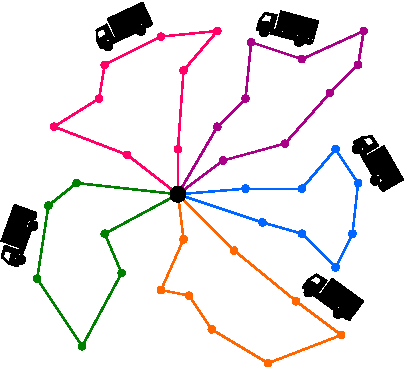
\includegraphics[height=4cm]{Imgs/CVRP-example.cropped.pdf}
		\end{column}
		\begin{column}{.65\textwidth}
			We are given:
			\begin{itemize}
				\item Customer \textcolor{blue}{locations} within a road network.
				\item The \textcolor{blue}{demand} of each customer.
				\item The \textcolor{blue}{vehicle capacity}.
				\item Number of \textcolor{blue}{available trucks}.
			\end{itemize}
			Objective:
			\begin{itemize}
				\item \textcolor{red}{Serve \textbf{all} customers while minimizing the overall routing cost}.
			\end{itemize}
		\end{column}
	\end{columns}

\end{frame}

\begin{frame}{Branch-price-and-cut}
\end{frame}

\begin{frame}{The Pricing Sub-problem}
	To advance the column generation, the \textcolor{blue}{pricer}, a critical component in BPC frameworks, needs to solve the \textcolor{blue}{pricing sub-problem} (PP):
	\begin{itemize}
		\item An \textcolor{blue}{Elementary Shortest Path Problem with Capacity Constraints} (\textbf{ESPPCC}) in a reduced cost network with negative cycles.
		      \begin{itemize}
			      \item NP-hard problem \parencite{dror1994}.
		      \end{itemize}
		\item \textbf{Relax elementarity condition} to make it solvable in pseudo-polynomial time:
		      \begin{itemize}
			      \item $q$-routes with 2-cycles elimination \parencite{christofides1969}.
			      \item $q$-routes with arbitrary $k$-cycles elimination \parencite{christofides1969}.
			      \item ng-routes \parencite{baldacci2011}.
		      \end{itemize}
		\item State-of-the-art solutions for the \textcolor{red}{relaxed} PP are based on \textcolor{blue}{dynamic programming}:
		      \begin{itemize}
			      \item \textbf{labeling algorithm} \parencite{desrochers1992, feillet2004}.
		      \end{itemize}
	\end{itemize}
\end{frame}

\begin{frame}{Thesis Contributions}
\end{frame}

\begin{frame}{Implementation}
\end{frame}

\begin{frame}{Empirical evaluation}
\end{frame}

\begin{frame}{Results (1/2)}

\end{frame}

\begin{frame}{Results (2/2)}

\end{frame}

\begin{frame}{Conclusions and Future Work}
	\cite{jepsen2014}
\end{frame}

\begin{frame}{The end}
	\begin{center}
		\begingroup
		\fontsize{18pt}{18pt}\selectfont
		Thank, you.
		\endgroup
	\end{center}
\end{frame}

\appendix

\begin{frame}
\end{frame}

\begin{frame}
	\begin{center}
		\begingroup
		\fontsize{18pt}{18pt}\selectfont
		Appendix.
		\endgroup
	\end{center}
\end{frame}

\begin{frame}{Integer Programming}
\end{frame}

\begin{frame}
	\maketitle
\end{frame}
